\subsection{SVM Inequality}
{\bf Proof of the inequality}
\begin{equation}
	P\Bigg\{ \sup_{ \vec{w} \in \Lambda  }
		\Big| R_{ ( \vec{w} ) } -
		  R_{ \mathrm{emp} ( \vec{w} ) }^{ (P) }
		\Big| > \eta
	\Bigg\} < 4 \exp \Bigg\{ H_{ \mathrm{ann} (2p) }^\Lambda 
			- p\Big( \eta - \frac{1}{p} \Big)^2
	\Bigg\}
\end{equation}
{\bf a) Nomenclature} \\\\
\noindent Consider two spot samples $1$ and $2$ of size $p$. Let
\begin{equation}
	R_{ \mathrm{emp} }^{ (p, 1) } = \frac{1}{p}
		\sum_{ \alpha = 1 }^p 
		Q_{ ( \mathrm{ \underline{Z} }^{ (\alpha ) }, 
		\vec{w} ) } 
\end{equation}
\begin{equation}
	R_{ \mathrm{emp} }^{ (p, 2) } = \frac{1}{p}
		\sum_{ \alpha = p + 1 }^{2p} 
		Q_{ ( \mathrm{ \underline{Z} }^{ (\alpha ) }, 
		\vec{w} ) }
\end{equation}
be the means of the costs for the samples $1$ and $2$, and
\begin{equation}
	\varphi_{ (2p) }^\Lambda = 
		\sup_{ \vec{w} \in \Lambda  }
	\underbrace{ \Big| 
		R_{ (\mathrm{emp} ( \vec{w} )  }^{ (p, 1) }
	-	R_{ \mathrm{emp} ( \vec{w} ) }^{ (p, 2) }
		\Big| }_{ \coloneqq 
			\varphi_{ (2p,\vec{w} ) }^\Lambda }
\end{equation}
be their difference, and
\begin{equation}
	\Pi_{ (p) }^\Lambda = 
		\sup_{ \vec{w} \in \Lambda  }
	\underbrace{ \Big| 
		R_{ ( \vec{w} ) } -
		R_{ \mathrm{emp} ( \vec{w} ) }^{ (p, 1) }
		\Big| }_{\coloneqq 
			\Pi_{ (p,\vec{w} ) }^\Lambda }
\end{equation}
be the difference between the mean and the expectation.\\\\
{\bf b) Lemma}
\begin{equation}
	P\Bigg\{ \Pi_{ (p) }^\Lambda > \eta \Bigg\}
	< 2P\Bigg\{ \varphi_{ (2p) }^\Lambda > \eta - \frac{1}{p} \Bigg\}
\end{equation}
\underline{Proof of the lemma:}\\
Let $A$ be the event
\begin{equation}
	A = \Big\{ \mathrm{ \underline{z} }, \ldots, 
		\mathrm{ \underline{z} }_p: 
		\Pi_{ (p) }^\Lambda > \eta\Big\}
\end{equation}
Let $\vec{w}^*$ be a model for which 
\begin{equation}
	\Pi_{ (p,\vec{w}^* ) }^\Lambda > \eta
\end{equation}
holds. Then the following will also hold,
\begin{equation}
	\begin{array}{ll}
	P\Big\{ \varphi_{ (2p) }^\Lambda > \eta - \frac{1}{p}\Big\}
	& = \int \mathrm{d} 
		F_{ \big( \mathrm{\underline{z}}, \ldots,
			\mathrm{\underline{z}}_{2p} \big) } 
		\Theta_{ \big( 
			\varphi_{ (2p) }^\Lambda - \eta + \frac{1}{p} 
			\big) } \\
	& = \int \mathrm{d} 
		F_{ \big( \mathrm{\underline{z}}_1, \ldots,
			\mathrm{\underline{z}}_{p} \big) }
		F_{ \big( \mathrm{\underline{z}}_{ p + 1 }, \ldots,
			\mathrm{\underline{z}}_{2p} \big) }
		\Theta_{ \big( 
			\varphi_{ (2p) }^\Lambda - \eta + \frac{1}{p} 
			\big) } \\
	& \geq \int_A \mathrm{d} 
		F_{ \big( \mathrm{\underline{z}}_1, \ldots,
			\mathrm{\underline{z}}_{p} \big) }
		F_{ \big( \mathrm{\underline{z}}_{ p + 1 }, \ldots,
			\mathrm{\underline{z}}_{2p} \big) }
		\Theta_{ \big( 
			\varphi_{ (2p) }^\Lambda - \eta + \frac{1}{p} 
			\big) } \\
	& \geq \int_A \mathrm{d} 
		F_{ \big( \mathrm{\underline{z}}_1, \ldots,
			\mathrm{\underline{z}}_{p} \big) }
	\underbrace{ F_{ \big( \mathrm{\underline{z}}_{ p + 1 }, \ldots,
			\mathrm{\underline{z}}_{p} \big) }
		 \Theta_{ \big( 
			\varphi_{ (2p, \vec{w}^* ) }^\Lambda 
			- \eta + \frac{1}{p} 
			\big) } }_{ \textrm{'inner' integral I} }
	\end{array}
\end{equation}
because the $\Theta$-function is $1$ over a great range, if a maximum over $\vec{w}$ is assumed.
\\\\
{\bf Estimate of the 'inner' integral I} \\\\
\noindent\textcircled{1}\\
Case $R_{ ( \vec{w}^* ) } - R_{ \mathrm{emp}( \vec{w}^* ) }^{ (p, 1) } > \eta$ of the constraint $\Pi_{ (p, \vec{w}^* ) }^\Lambda > \eta$.\\\\
Let $R_{ \mathrm{emp}( \vec{w}^* ) }^{ (p, 2) } > R_{ ( \vec{w}^* ) } - \frac{1}{p}$ hold, then
\begin{equation}
	R_{ \mathrm{emp}( \vec{w}^* ) }^{ (p, 2) } 
	- R_{ \mathrm{emp}( \vec{w}^* ) }^{ (p, 1) }
	> R_{ ( \vec{w}^* ) } - \frac{1}{p} 
	- R_{ \mathrm{emp}( \vec{w}^* ) }^{ (p, 1) }
	> \eta - \frac{1}{p}
\end{equation}
\begin{equation}
	R_{ \mathrm{emp}( \vec{w}^* ) }^{ (p, 1) } 
	- R_{ \mathrm{emp}( \vec{w}^* ) }^{ (p, 2) }
	< R_{ \mathrm{emp}( \vec{w}^* ) }^{ (p, 1) }
	- R_{ ( \vec{w}^* ) } + \frac{1}{p} 
	< -\eta + \frac{1}{p}
\end{equation}
follows. Therefore
\begin{equation}
	\varphi_{ (2p, \vec{w}^* ) }^\Lambda = 
	\Big| R_{ \mathrm{emp}( \vec{w}^* ) }^{ (p, 1) } 
	- R_{ \mathrm{emp}( \vec{w}^* ) }^{ (p, 2) } \Big|
	> \eta - \frac{1}{p}
\end{equation}
Which means
\begin{center}
	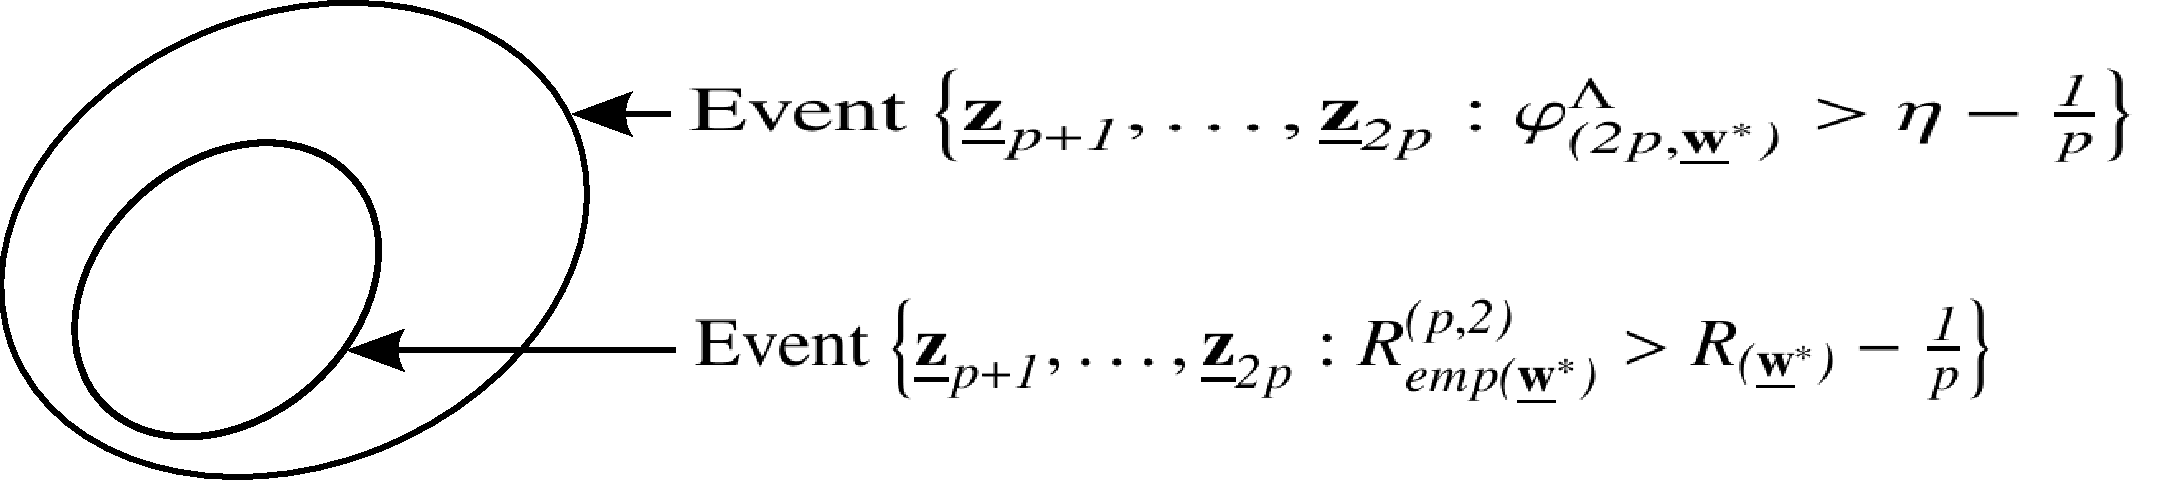
\includegraphics[width=8cm]{proofSVMinequality-fig1}
\end{center}
Now consider the event $\Big\{ \mathbf{ \underline{z}}_{p+1}, \ldots, \mathbf{ \underline{z}}_{2p} : R_{ \mathrm{emp}( \vec{w}^* ) }^{ (p, 2) } > R_{ ( \vec{w}^* ) } - \frac{1}{p} \Big\}$ :
\begin{equation}
	R_{ \mathrm{emp}( \vec{w}^* ) }^{ (p, 2) }
	= \frac{1}{p} \sum_{ \alpha = p + 1 }^{2p} 
		Q_{ ( \mathrm{ \underline{Z} }^{ (\alpha ) }, 
		\vec{w}^* ) }
	> R_{ ( \vec{w}^* ) } - \frac{1}{p}
\end{equation}
\begin{equation}
	\sum_{ \alpha = p + 1 }^{2p} 
		Q_{ ( \mathrm{ \underline{Z} }^{ (\alpha ) }, 
		\vec{w}^* ) }
	> pR_{ ( \vec{w}^* ) } - 1
\end{equation}
The inequality holds, if the number $k$ of ones in the sum on the left hand is greater than the value on the right hand.
\begin{equation}
	k > pR_{ ( \vec{w}^* ) } - 1
\end{equation}
Probability $P_{(k)}$, that the above sum consists of $k$ ones.\\
$\leadsto R_{ ( \vec{w}^* ) }$ is the probability that $Q_{ ( \mathrm{ \underline{Z} }^{ (\alpha ) },	\vec{w}^* ) } = 1$\\
$\leadsto$ observed data is iid
\begin{equation}
	P_{ (k) } = \rmat{p\\k} R_{ ( \vec{w}^* ) }^k 
		\Big( 1 - R_{ ( \vec{w}^* ) } \Big)^{p-k}
\end{equation}
which is the binominal distribution.
\begin{center}
	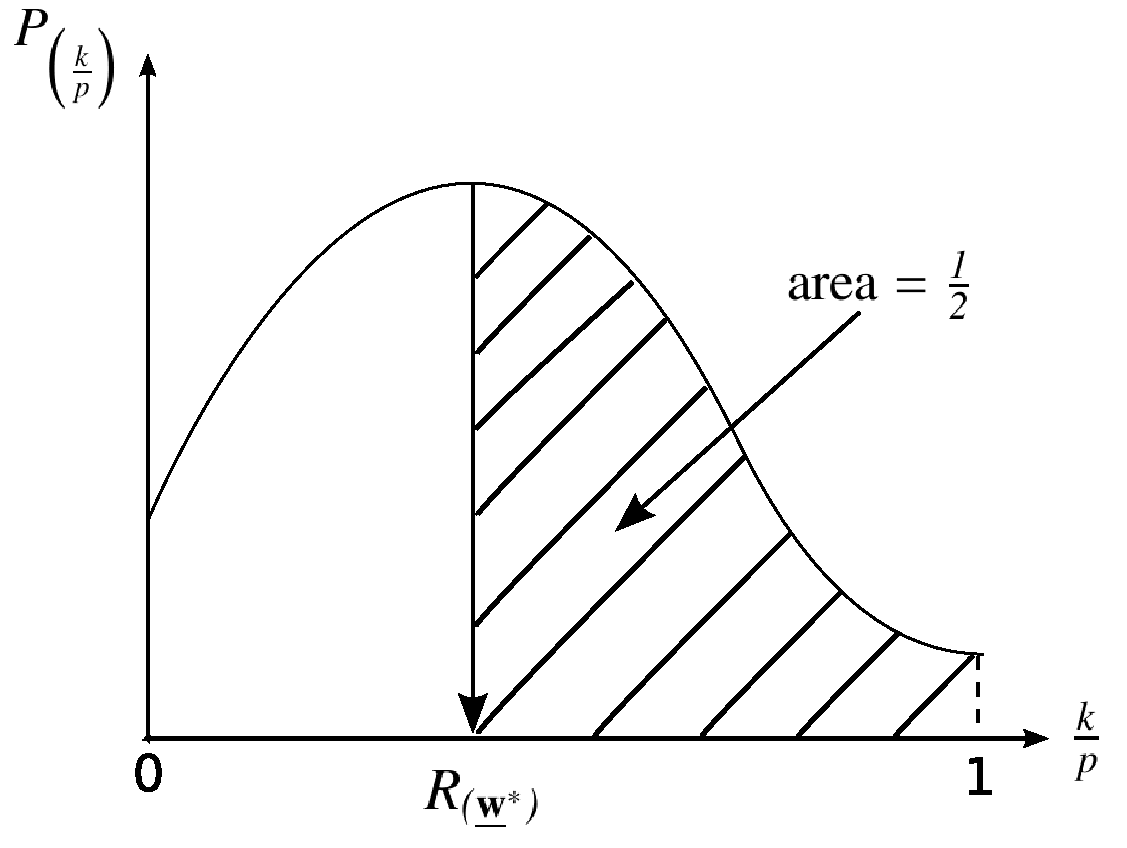
\includegraphics[width=6cm]{proofSVMinequality-fig2}
\end{center}
With this we get the following for the 'inner' integral I (with a restriction to a less powerful event)
\begin{equation}
	\begin{array}{ll}
	I
	& \geq \int \mathrm{d} 
		F_{ \big( \mathrm{\underline{z}}_{p + 1}, \ldots,
			\mathrm{\underline{z}}_p \big) } 
		\Theta_{ \big( R_{ \mathrm{emp} }^{ (p, 2) } -
			R_{ ( \vec{w}^* ) } + \frac{1}{p} 
		\big) } \\
	& = P\Bigg\{ R_{ \mathrm{emp} ( \vec{w}^* ) 
			}^{ (p, 2) }
			> R_{ ( \vec{w}^* ) } - \frac{1}{p} 
		\Bigg\} \\
	& > \frac{1}{2}
	\end{array}
\end{equation}
follows from the property of the binominal distribution.\\\\
\textcircled{2}\\
Case $R_{ ( \vec{w}^* ) } - R_{ \mathrm{emp}( \vec{w}^* ) }^{ (p, 1) } < -\eta$ of the constraint $\Pi_{ (p, \vec{w}^* ) }^\Lambda > \eta$.\\\\
Let $R_{ \mathrm{emp}( \vec{w}^* ) }^{ (p, 2) } < R_{ ( \vec{w}^* ) } + \frac{1}{p}$ hold, then
\begin{equation}
	R_{ \mathrm{emp}( \vec{w}^* ) }^{ (p, 2) } 
	- R_{ \mathrm{emp}( \vec{w}^* ) }^{ (p, 1) }
	< R_{ ( \vec{w}^* ) } + \frac{1}{p} 
	- R_{ \mathrm{emp}( \vec{w}^* ) }^{ (p, 1) }
	< -\eta + \frac{1}{p}
\end{equation}
\begin{equation}
	R_{ \mathrm{emp}( \vec{w}^* ) }^{ (p, 1) } 
	- R_{ \mathrm{emp}( \vec{w}^* ) }^{ (p, 2) }
	> R_{ \mathrm{emp}( \vec{w}^* ) }^{ (p, 1) }
	- R_{ ( \vec{w}^* ) } - \frac{1}{p} 
	> \eta - \frac{1}{p}
\end{equation}
follows. Also
\begin{equation}
	\varphi_{ (2p, \vec{w}^* ) }^\Lambda = 
	\Big| R_{ \mathrm{emp}( \vec{w}^* ) }^{ (p, 1) } 
	- R_{ \mathrm{emp}( \vec{w}^* ) }^{ (p, 2) } \Big|
	> \eta - \frac{1}{p}
\end{equation}
In analogy to case \textcircled{1} we begin by estimating the probability of the event:
\begin{equation}
	\Bigg\{ \mathrm{ \underline{z}_{p + 1} }, \ldots, 
		\mathrm{ \underline{z} }_{2p}: 
		R_{ \mathrm{emp}( \vec{w}^* ) }^{ (p, 2) }
		< R_{ ( \vec{w}^* ) } + \frac{1}{p}
	\Bigg\}
\end{equation}
and we get the following for the 'inner' integral (with a restriction to a less powerful event)
\begin{equation}
	\begin{array}{ll}
	I
	& \geq \int \mathrm{d} 
		F_{ \big( \mathrm{\underline{z}}_{p + 1}, \ldots,
			\mathrm{\underline{z}}_{2p} \big) } 
		\Theta_{ \Big( R_{ ( \vec{w}^* ) } 
			+ \frac{1}{p} 
			- R_{ \mathrm{emp} ( \vec{w}^* ) 
				}^{ (p, 2) }
			\Big) } \\
	& = P\Bigg\{ R_{ \mathrm{emp} ( \vec{w}^* ) }
			^{ (p, 2) }
			< R_{ ( \vec{w}^* ) } + \frac{1}{p} 
		\Bigg\} \\
	& > \frac{1}{2}
	\end{array}
\end{equation}
again, according to the properties of the binominal distribution.\\\\
Finally, it follows from case \textcircled{1} and \textcircled{2}
\begin{equation}
	P\Bigg\{ \varphi_{ (2p) }^\Lambda > \eta - \frac{1}{p} \Bigg\}
	> \frac{1}{2} \int_A \mathrm{d} 
		F_{ \big( \mathrm{\underline{z}}_1, \ldots,
			\mathrm{\underline{z}}_{p} \big) }
	= \frac{1}{2} P\Bigg\{ \Pi_{ (p) }^\Lambda > \eta \Bigg\}
\end{equation}
{\bf c) A useful estimation}
\\\\
Given:
\begin{equation}
	\Gamma = \sum_{ k \in K } 
		\frac{ \rmat{m\\k} \rmat{2p-m\\p-k} }{ \rmat{2p\\p} }
\end{equation}
\begin{equation}
	K = \Bigg\{ k: \Big| k - \frac{m}{2} \Big| > \frac{\varepsilon p}{2}
		\textrm{ and }
		\max(0, m-p) \leq k \leq \min(m, p)
		\Bigg\}
\end{equation}
Goal: Find an upper boundary for $\Gamma$. \\
Let $\Gamma = \Gamma_1 + \Gamma_2$ with
\begin{equation}
	\Gamma_1 = \sum_{ k \in K_1 } 
		\frac{ \rmat{m\\k} \rmat{2p-m\\p-k} }{ \rmat{2p\\p} }
	\textrm{ for } k > \frac{m}{2} + \frac{\varepsilon p}{2}
\end{equation}
\begin{equation}
	\Gamma_1 = \sum_{ k \in K_2 } 
		\frac{ \rmat{m\\k} \rmat{2p-m\\p-k} }{ \rmat{2p\\p} }
	\textrm{ for } k < \frac{m}{2} - \frac{\varepsilon p}{2}
\end{equation}
Now we will make estimations for $\Gamma_1$ and $\Gamma_2$.\\\\
\textcircled{1}\\
Nomenclature:
\begin{equation}
	P_{(k)} = \frac{ \rmat{m\\k} \rmat{2p-m\\p-k} }{ \rmat{2p\\p} }
\end{equation}
\begin{equation}
	q_{(k)} = \frac{P_{(k+1)}}{P_{(k)}} 
		= \frac{ (m-k)(p-k) }{ (k+1)(p+k+1-m) }
\end{equation}
\begin{equation}
	s = \min(m, p)
\end{equation}
\begin{equation}
	d_{(j)} = \sum_{k = j}^s P_{(k)}
\end{equation}
$j^*$: lowest number, with $j^* > \frac{m}{2} + \frac{\varepsilon p}{2}$\\\\
To be estimated: $\Gamma_1 = d_{ (j^*) }$.\\\\
Relations for $d_{ (j) }$:
\begin{equation}
	d_{ (j + 1) } = \sum_{ k = j + 1 }^s P_{ (k) }
	= \sum_{ k = j }^{ s - 1 } P_{ (k + 1) }
	= \sum_{ k = j }^{ s - 1 } P_{ (k) } q_{ (k) }
	< q_{ (j) } \sum_{ k = j }^{ s - 1 } P_{ (k) }
	< q_{ (j) } \sum_{ k = j }^{ s }
	= q_{ (j) } d_{ (j) }
\end{equation}
with recursive application we gain:
\begin{equation}	
	d_{ (j) } < d_{ (i) } \Pi_{ k = i }^{j - 1} q_{ (k) }
		< \Pi_{ k = i }^{j - 1} q_{ (k) }
		\textrm{ because of } d_{ (i) } < 1
\end{equation}
Relations for $q_{ (k) }$:
\begin{equation} 
	t = k - \frac{m - 1}{2}
\end{equation}
$\leadsto |t| < \min \Big( \frac{m + 1}{2}, p - \frac{m - 1}{2}	\Big)$\\
$\leadsto k = t + \frac{m - 1}{2}$
\begin{equation}
	q_{ (t) } = \frac{ \frac{m + 1}{2} - t }{ \frac{m + 1}{2} + t } \cdotp 
		\frac{ \Big(p - \frac{m - 1}{2} \Big) - t }
			{ \Big(p - \frac{m + 1}{2} \Big) + t }
\end{equation}
\underline{Auxiliary calculation to estimate $q_{ (t) }$:}
\begin{equation}
	F_{ (t) } = \frac{ a - t }{ a + t } \cdotp \frac{ b - t }{b + t },
	\textrm{ with } a,b > 0 \textrm{ and } |t| < \min(a,b)
\end{equation}
\begin{equation}
	\ln F_{ (t) } = \ln (a - t) - \ln (a + t) + \ln (b - t) - \ln (b + t)
\end{equation}
\begin{equation}
	\ln F_{ (0) } = 0
\end{equation}
\begin{equation}
	\begin{array}{ll}
	\frac{ \mathrm{d} }{ \mathrm{d}t } (\ln F_{ (t) })
	& = -\frac{1}{ a - t } -\frac{1}{ a + t }
		-\frac{1}{ b - t }-\frac{1}{ b + t } \\\\
	& = -\Big( \frac{ 2a }{ a^2 - t^2 } + \frac{ 2b }{ b^2 - t^2 }
		\Big) \\\\
	& \leq -2\Big( \frac{1}{a} + \frac{1}{b} \Big)
	\textrm{ for } |t| < \min(a,b)	\\\\
	\end{array}
\end{equation}
\begin{equation}
	\ln F_{ (t) } \leq -2\Big( \frac{1}{a} + \frac{1}{b} \Big) t
	\textrm{ after integrating the boundary}
\end{equation}
\begin{equation}
	\ln q_{ (t) } \leq -2\Bigg( \frac{ 2 }{ m + 1 } 
		+ \frac{ 2 }{ 2p - m + 1 } \Big) t
	= -8 \frac{ p + 1 }{ (m + 1)(2p - m + 1) }t
\end{equation}
Estimation of $d_{(j)}$:
\begin{equation}
	\ln d_{(j)} = \ln \Pi_{ k = i }^{j - 1} q_{ (k) }
	= \sum_{ k = i }^{j - 1} \ln q_{ (k) }
	\leq -8 \frac{ p + 1 }{ (m + 1)(2p - m + 1) } \sum_{ k = i }^{j - 1}
		\Big( k - \frac{ m - 1 }{2} \Big)
\end{equation}
For an even $m$, choose an $i$, so that:
\begin{equation}
	i = \frac{m}{2} \leadsto \sum_{ k = \frac{m}{2} }^{j - 1}
		\Bigg( k - \frac{ m - 1 }{2} \Bigg)
		= \frac{1}{2} \Bigg( j - \frac{m}{2} \Bigg)^2
\end{equation}
For an odd $m$, choose an $i$, so that:
\begin{equation}
	i = \frac{ m - 1 }{2} \leadsto \sum_{ k = \frac{ m - 1 }{2} }^{j - 1}
		\Bigg( k - \frac{ m - 1 }{2} \Bigg)
		= \frac{1}{2} \Bigg( j - \frac{ m - 1 }{2} \Bigg)
			\Bigg( j - \frac{ m - 1 }{2} - 1 \Bigg)
		< \frac{1}{2} \Bigg( j - \frac{ m - 1 }{2} \Bigg)^2
\end{equation}
\begin{equation}
	\ln d_{ (j) } < \frac{ 4 (p + 1) }{ (m + 1)(2p - m + 1) }
		\Bigg( j - \frac{ m - 1 }{2} \Bigg)
\end{equation}
\underline{Estimation of $\Gamma_1$}:
\begin{equation}
	\ln \Gamma_1 < \frac{ p + 1 }{ (m + 1)(2p - m + 1) } \varepsilon^2 p^2
	\textrm{ because of } j^* - \frac{ m }{ 2 } > \frac{\varepsilon p}{2}
\end{equation}
Maximizing the right hand side:
\begin{equation}
	\frac{ \mathrm{d} }{ \mathrm{d}m } \cdotp
		\frac{ 1 }{ (m + 1)(2p - m + 1) } 
	= \frac{ 2p - m + 1 - m - 1 }{ (m + 1)^2 (2p - m + 1)^2 }
	= 2\frac{ p - m }{ (m + 1)^2 (2p - m + 1)^2 } \eqexcl 0 
\end{equation}
$m \eqexcl p$, is the maximum because the change of sign turned from positive $\rightarrow$ negative for $m\uparrow$.
\begin{equation}
	\ln \Gamma_1 < -\frac{ \varepsilon^2 p^2 }{ p + 1 } < -\varepsilon^2 p
\end{equation}
\begin{equation}
	\Gamma_1 < \exp\big( -\varepsilon^2 p\big)
\end{equation}
\textcircled{2}\\
Estimation of the partial sum $\Gamma_2$
\begin{equation}
	P_{ (k) } = \frac{ \rmat{m\\k} \rmat{2p-m\\p-k} }{ \rmat{2p\\p} }
\end{equation}
\begin{equation}
	k = \frac{m}{2} + t
\end{equation}
\begin{equation}
	P_{ (t) } = \rmat{2p\\p}^{-1} \rmat{m\\\frac{m}{2}+t} 
			\rmat{2p-m\\p-\frac{m}{2}+t}
		= \Big( \frac{2p}{p} \Big)^{-1} 
			\frac{ m\mathrm{!} ( 2p - m )\mathrm{!} }
			{ \Big( \frac{m}{2} + t \Big)\mathrm{!}
			  \Big( \frac{m}{2} - t \Big)\mathrm{!}
			  \Big( p - \frac{m}{2} + t \Big)\mathrm{!}
			  \Big( p - \frac{m}{2} - t \Big)\mathrm{!} }
\end{equation}
$\Rightarrow$ Symmetry $P_{ (t) } = P_{ (-t) }$\\
Therefore
\begin{equation}
	\Gamma_2 = \Gamma_1 < \exp \big(-\varepsilon^2 p\big)
\end{equation}
\underline{Synopsis:}\\\\
\begin{equation}
	\Gamma = \Gamma_1 + \Gamma_2 < 2\exp \big(-\varepsilon^2 p \big)
\end{equation}
{\bf Proof of the theorem} 
\\\\
Because of the lemma it is sufficient to estimate an upper bound for
\begin{equation} \label{main}
	P\Big\{ \varphi_{ (2p) }^\Lambda > \eta - \frac{1}{p} \Big\}
\end{equation}
Let $T_i^{ (2p) }, i \in \big\{ 1, \ldots, 2_p \big\}$ be a random permutation of the sequence of the $2p$ observed data points. Because the probability (\ref{main}) is independent of the order of the observations the following holds:
\begin{equation}
	\begin{array}{ll}
	P\Big\{ \varphi_{ (2p) }^\Lambda > \eta - \frac{1}{p}\Big\}
	& = \int \mathrm{d} 
		F_{ \big( \mathrm{\underline{z}}_1, \ldots,
			\mathrm{\underline{z}}_{2p} \big) } 
		\Theta_{ \Big( 
			\varphi_{ (2p) }^\Lambda - \eta + \frac{1}{p} 
			\Big) } \\	
	& = \int \mathrm{d} 
		F_{ \big( \mathrm{\underline{z}}_1, \ldots,
			\mathrm{\underline{z}}_p \big) } 
		\frac{1}{ ( 2p ) \mathrm{!} }
		\sum_{i = 1}^{ 2p }
		\Theta_{ \bigg( 
			\varphi_{ \big( T_i^{ (2p) } \big) }^\Lambda 
			- \eta + \frac{1}{p} \bigg) } \\
	& = \int \mathrm{d} 
		F_{ \big( \mathrm{\underline{z}}_1, \ldots,
			\mathrm{\underline{z}}_p \big) } 
		\frac{1}{ ( 2p ) \mathrm{!} }
		\sum_{i = 1}^{ 2p }
		\Theta_{ \bigg( \sup_{ \vec{w} \in \Lambda } 
			\varphi_{ \big( T_i^{ (2p) },
				\vec{w}
			\big) }^\Lambda 
			- \eta + \frac{1}{p} \bigg) } \\
	& = \int \mathrm{d} 
		F_{ \big( \mathrm{\underline{z}}_1, \ldots,
			\mathrm{\underline{z}}_p \big) } 
		\frac{1}{ ( 2p ) \mathrm{!} }
		\sum_{i = 1}^{ 2p }
		\sup_{ \vec{w} \in \Lambda }
		\Theta_{ \bigg(  
			\varphi_{ \big( T_i^{ (2p) },
				\vec{w}
			\big) }^\Lambda 
			- \eta + \frac{1}{p} \bigg) }
	\end{array}
\end{equation}
Let $\Lambda_{ \big( \mathrm{ \underline{z}_1 }, \ldots, \mathrm{ \underline{z}_{2_p} } \big) }^* \subset \Lambda$ be a set of all possible on the dataset's $\big\{ \underline{Z}_1, \ldots, \underline{Z}_p \big\}$ distinguishable functions $\vec{w}^*$.\\
Then the following holds:
\begin{equation}
	\begin{array}{ll}
	P\Big\{ \varphi_{ (2_p) }^\Lambda > \eta - \frac{1}{p}\Big\}
	& = \int \mathrm{d} 
		F_{ \big( \mathrm{\underline{z}}_1, \ldots,
			\mathrm{\underline{z}}_{2p} \big) }
		\sup_{ \vec{w}^* \in \Lambda^* }
		\frac{1}{ ( 2_p ) \mathrm{!} }
		\sum_{i = 1}^{ 2p }
		\Theta_{ \bigg( 
			\varphi_{ \big( T_i^{ (2p) }, \vec{w}^* 
			\big) }^\Lambda 
			- \eta + \frac{1}{p} \bigg) } \\
	& \leq \int \mathrm{d} 
		F_{ \big( \mathrm{\underline{z}}_1, \ldots,
			\mathrm{\underline{z}}_p \big) }
		\sum_{ \vec{w}^* \in \Lambda^* }
		\frac{1}{ ( 2_p ) \mathrm{!} }
		\sum_{i = 1}^{ 2p }
		\Theta_{ \bigg( 
			\varphi_{ \big( T_i^{ (2p) }, \vec{w}^* 
			\big) }^\Lambda 
			- \eta + \frac{1}{p} \bigg) } \\
	\end{array}
\end {equation}
$m$: number of data points $\underline{z} \in \big\{ \underline{z}_1, \ldots, \underline{z}_p \big\}$ for which $Q_{ ( \underline{z}, \mathbf{\underline{w}^* } ) } = 1$\\
$k$: number of data points $\underline{z}$ from $R_{ \mathrm{emp} (\mathbf{\underline{w}}^*)}$ for which $Q_{ \underline{z}, \mathbf{\underline{w}^* } ) } = 1$
\begin{equation}
	\Theta_{ \bigg( 
			\varphi_{ \big( T_i^{ (2p) }, \vec{w}^* 
			\big) }^\Lambda 
			- \eta + \frac{1}{p} \bigg) }
	\Rightarrow 1 \textrm{ iff } \Big| 
	\underbrace{ \frac{k}{p} }_{ R_{ \mathrm{emp} 
		( \mathbf{\underline{w}^*) } }^{ (p,1) } }
	-\underbrace{ \frac{m-k}{p} }_{ R_{ \mathrm{emp} 
		( \mathbf{\underline{w}^*) } }^{ (p,2) } } \Big|
	> \eta -\frac{1}{p}
\end{equation}
In the following we will denote the set of all $k$, for which the above statement holds, by $K$.\\\\
Estimation of the integral:
\begin{equation}
	\begin{array}{ll}
		\Gamma 
		& = \frac{1}{ ( 2_p ) \mathrm{!} } \sum_{ i = 1 }^{ 2p }
		  \Theta_{ \bigg( 
			\varphi_{ \big( T_i^{ (2p) }, \vec{w}^* 
			\big) }^\Lambda 
			- \eta + \frac{1}{p} \bigg) } \\\\
		& = \frac{ \textrm{number of permutations for which }
			\bigg( \varphi_{ \big( T_i^{ (2p) }, 
				\vec{w}^* \big) }^\Lambda 
			> \eta - \frac{1}{p} \bigg)
			\textrm{ holds.} }{ \textrm{number of all permutations}}
			\\\\
		& = \frac{1}{ ( 2_p ) \mathrm{!} } \sum_{ k \in K } 
			m\mathrm{!} (2p-m)\mathrm{!} 
			\frac{p \cdotp \ldots \cdotp p-k+1 }
				{k \mathrm{!}}
				\cdotp \frac{p \cdotp \ldots \cdotp p-m+k+1 }
				{(m-k) \mathrm{!}} \\\\
		& = \sum_{k \in K} \frac{ m\mathrm{!} }{ k\mathrm{!} 
			(m-k) \mathrm{!}} \cdotp \frac{(2p-m) \mathrm{!} }{
				(p-k) \mathrm{!} (p-m+k) \mathrm{!} }
			\cdotp \frac{p\mathrm{!}p\mathrm{!}}{
				(2p)\mathrm{!}} \\\\
		& = \sum_{k \in K} \frac{ \rmat{m\\k} \rmat{2p-m\\p-k} }{
			\rmat{2p\\p}}
	\end{array}
\end{equation}
Notes:\\
$m\mathrm{!}$: permutation of $m$ data points $\leadsto Q_{ ( \mathrm{\underline{z}}, \vec{w}^* )} = 1$\\
$(2p-m)\mathrm{!}$: permutations of $2p - m$ data points $\leadsto Q_{ ( \mathrm{\underline{z}}, \vec{w}^* )} = 0$\\
$k\mathrm{!}$: number of distinct binary sequences of length $p$ with $k$ 'ones'\\
$(m-k) \mathrm{!}$: number of distinct sequences of length $p$ with $m - k$ 'ones'\\
As we have shown in c), the following holds:
\begin{equation}
	\Gamma = \sum_{k \in K} \frac{ \rmat{m\\k} \rmat{2p-m\\p-k} }{
			\rmat{2p\\p}} < 2\exp\Bigg\{ -\Big( \eta -\frac{1}{2}
			\Big)^2 p\Bigg\}
\end{equation}
Therefore
\begin{equation}
	\begin{array}{ll}
	P\Big\{ \varphi_{ (2p) }^\Lambda > \eta - \frac{1}{p}\Big\}
	& = \int \mathrm{d} 
		F_{ \big( \mathrm{\underline{z}}_1, \ldots,
			\mathrm{\underline{z}}_{2p} \big) }
		\sum_{ \vec{w}^* \in \Gamma^* }
		\Gamma \\\\
	& < 2\exp\Bigg\{ -\Big( \eta -\frac{1}{2} \Big)^2 p\Bigg\}
		\int \mathrm{d} F_{ \big( \mathrm{\underline{z}}_1, \ldots,
			\mathrm{\underline{z}}_{2p} \big) }
		N_{ \big( \mathrm{\underline{z}}_1, \ldots,
			\mathrm{\underline{z}}_{2p} \big) }^\Lambda \\\\
	& = 2\exp\Bigg\{ H_{ ann (2p) }^\Lambda 
		- \Big( \eta -\frac{1}{2} \Big)^2 p\Bigg\}
	\end{array}
\end{equation}
And finally, together with the result from the lemma in b)
\begin{equation}
	P\Big\{ \Pi_{ (p) }^\Lambda > \eta \Big\}
	< 4\exp\Bigg\{ H_{ ann (2p) }^\Lambda 
		- \Big( \eta -\frac{1}{2} \Big)^2 p\Bigg\}
\end{equation}
